243. \begin{figure}[ht!]
\center{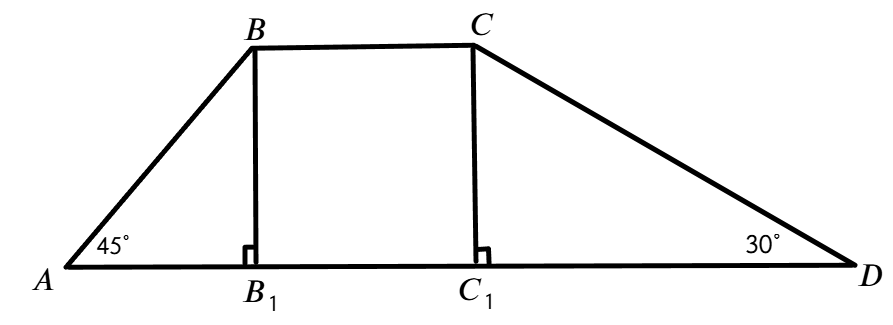
\includegraphics[scale=0.35]{g8-239.png}}
\end{figure}\\
Найдём $AB_1=BB_1 ctg(45^\circ)=4$ и $DC_1=CC_1 ctg(30^\circ)=4\sqrt{3}.$ Так как $BCC_1B_1$ является прямоугольником, $B_1C_1=BC$ и верно соотношение
$S_{ABCD}=\cfrac{1}{2}\cdot4\cdot(BC+BC+4+4\sqrt{3})=32,$ откуда $2BC+4+4\sqrt{3}=16,\ BC=6-2\sqrt{3}.$\\
